\chapter{Axions in Cosmology}


With the advent of precision cosmology, particle physicists can use the entire universe as a laboratory for ever more sensitive experiments.
Of special interest is the axion's promise as a dark matter candidate.
We expect axions to be produced in astrophysical plasma, and therefore to possibly have significant implications on the evolution of the universe and of astrophysical structures.

Many cosmological tests of axion-like particles involve predicting relative particle abundances in the universe at various epochs, such as the baryon-to-photon or neutrino-to-photon ratios.
Such arguments begin with a minimal `thermodynamical' model of the universe as a homogeneous, isotropic, expanding background upon which different particle species exist uniformly distributed and in thermal equilibrium.
The universe's macrostate is characterised by each species' abundance and energy distribution, and can be given a cosmological temperature, $T$, quantifying average energy density.
Interactions and processes between species, which at any time may depend on present particle abundances and energies, define differential relations which can be solved to determine the abundance of each species at any point in the universe's evolution.


\begin{figure}[b!]
\begin{aside}[Terminology from cosmology]
\begin{itemize}[leftmargin=0.75em]\setlength\itemsep{0.25ex}
	\item \emph{thermalisation}
---	the process of a particle species reaching thermal equilibrium (i.e., uniform energy and abundance) over cosmological scales, mitigated by energy-diffusing self-interactions or processes with other species.
	\item \emph{freeze-out}
---	the point beyond which the rates of thermalising processes become negligible due to cooling cosmological temperature or accelerating cosmic expansion. Freeze-out results in persistent non-equilibrium distributions of a particle species, analogous to a change of phase from a gas to a cooler condensate.
% Since the universe cools as it expands, freeze-out may be viewed as a species' change of phase from a gas to a cooler condensate.
\end{itemize}
\end{aside}
\end{figure}

The assumptions of isotropy and homogeneity specify a spacetime with a Friedmann--Lemaître--Robertson--Walker (FLRW) metric,
\begin{align}
	% \ts g = -c^2 \ts\dd t\otimes\ts\dd t + a(t)^2\qty(η_{ij}\,\ts\dd x^i\otimes\ts\dd x^j)
	\ts g = -c^2 \ts\dd t^2 + a(t)^2\qty(\frac{\ts\dd r^2}{1 - kr^2} + r^2 \ts Θ)
\end{align}
where $k \in \qty{+1, 0, -1}$ reflects the type of spatial curvature, $\ts Θ = \ts\dd θ^2 + \sinθ\,\ts\dd φ^2$ is the metric of the unit sphere, and $\ts\dd x^2 \equiv \ts\dd x\otimes\ts\dd x$.
Standard cosmological models have flat spatial curvature, $k = 0$.
The scale factor $a(t)$ describes the cosmological evolution of the universe and defines the \emph{Hubble parameter,} $H \coloneqq \dot{a}/a$, or cosmic expansion rate.
If the rate $Γ$ of a particle interaction is large (corresponding to large probability per unit spacetime volume for the interaction to occur), then it will provide a mechanism for thermalisation of the species involved---or in the case of production and decay processes, will drive the species to abundance or extinction. 
If the rate is smaller than the rate of cosmic expansion, $Γ \ll H$, then the interaction or process will freeze-out and become negligible.
If a species' most dominant interactions freeze-out, then it becomes thermally isolated from other fields and its abundance remains fixed.





\section{Axion Interactions and Processes}


Axions decay into photons via the axion-photon vertex at a rate
\begin{align}
	Γ_{a\to 2γ} = \frac{g_{aγγ}^2m_a^3}{64π} \approx 10^{-24}\,\si{\per\second}\qty(\frac{m_a}{\si{\eV}})^5
,\end{align}
where the coupling strength $g_{aγγ}$ can be approximately written in terms of the mass given, with an $\cal O(1)$ model dependence \cite{Cadamuro_2011}.
Thus, for axions to exist in significant abundance in the present, they must be sufficiently light, or else the decay process dominates.
An inverse decay process $2γ \to a$ is also possible, with a rate $Γ_{2γ \to a} \propto 1/T$ increasing as the universe cools.
This implies that axions may recouple to photons at late stages of the universe's evolution \cite{Marsh_2016}.

Axions also interact by the strong force with hadronic matter via the gluon-axion vertex, giving rise to the Primakoff (and Compton) electron scattering processes shown in figure~\ref{fig:scattering-processes}.
When the universe is sufficiently hot so as to produce axions, $T \gg m_a$, the rate of Primakoff scattering $Γ_\text{P} \propto g_{aγγ}^2n_e$ is proportional to the number density of electrons-plus-positions, $n_e$ \cite{Cadamuro_2011}.
For leptonic (e.g., DFSZ) axions, \cite{Cadamuro_2011} approximate the rate of Compton scattering as
\begin{align}
	Γ_\text{C} \propto \frac{g_{aee}^2n_e}{\max\qty{T^2, m_a^2}}
.\end{align}
These scattering processes, along with photon decay and inverse decay, are the dominant interactions relevant to cosmology.
The freeze-out temperatures of these processes vary non-linearly with axion mass.

\begin{figure}
	\centering
	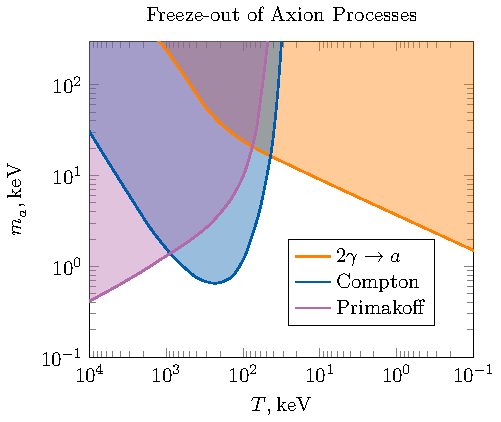
\includegraphics{diagrams/cosmo-freeze-out.pdf}
	\caption{
		Axion decoupling and recoupling with varying cosmological temperature.
		The evolution of the universe progresses from left-to-right, in the direction of \emph{decreasing} temperature.
		The shaded regions indicate periods where each processes occurred with ease, keeping axions thermalised.
	}
\end{figure}